\section{Hubbard model}

The nearly free electron gas models the conduction bands of metals and alloys fairly accurately. The high mobility of the electrons compared to the ions justifies two equivalent approximations, both giving essentially the same results\cite{Ashcroft1976}. The first idea is to treat the periodic potential created by the \emph{virtually} fixed ions (compared to the electrons) as a perturbation on the free electron gas. The other way of arriving at similar results is to imagine the system as a collection of tightly bond atoms, in which the higher energy conduction electrons hop from atom to atom. Both these approaches lead to band theory, a framework which allows us to predict whether a material is a conductor or a insulator. From the tight binding point of view, the effect of the electron mobility is the broadening of the atomic energy levels: the electrons in the solid occupy energy bands, rather than levels. The partially filled band of highest energy is called the conduction band, since it is the band occupied by conduction electrons hopping from atom to atom. However, in transition and rare-earth metals, there are partially filled bands other than to the conduction bands: $d-$ or $f-$bands. The partial filling of these bands and the electron correlations within them are responsible for the characteristic properties of these solids. Some of these properties are not explained by band theory, namely the Mott metal-insulator transition\cite{Boer1937, Mott1939, Mott1949}

Take Molybdenum, a transition metal. Its electronic configuration is $[Kr] 5s^1 4d^5$. The $s$-orbital is higher in energy than the $d$-orbital. Thus, the Fermi energy lies in the corresponding partially filled $s-$band, which is then the conduction band. However, the $d$-band will be only partially filled as well, leading to the effects mentioned in the previous paragraph. Platinum is yet another example, with electronic configuration $[Xe]4f^{14} 5d^9 6s^1 $, where the $5d$ level in only partially filled. In these partially filled narrow energy bands correlation phenomena are particularly relevant, as opposed to the case of conduction bands. Thus, the nearly free electron gas model does not suffice to describe the electrons in these bands; we must turn to a model that includes correlations. While for $f-$electrons of rare earth metals, a purely atomic, localized model - such as the Heitler-London model - might be satisfactory, the same cannot be said for $d-$electrons of transition metals because the band they occupy is narrower and correlations should be more relevant since the electronic states within the band are closer in energy.

\subsection{Electron correlations in narrow $d-$bands}

First, note that the effects of correlations cannot possibly be the same in narrow energy bands and in the free electron gas. To see this, we may simply recall the shape of a $d-$wave function. In a $d-$orbital, the electron charge density is concentrated near the nucleus. In a solid the electronic charge density should then also be concentrated near the nuclei, as long as the atomic description is useful, even if not completely correct\footnote{The electronic charge density is, of course, not actually defined in terms of a squared norm of the $d-$wave function for a narrow band. There is some broadening of the corresponding atomic energy level, and the wave function describing an electron is a Bloch wave function. Since the band is narrow, we assume that the atomic wave function description is still somewhat useful in a given range and we use it to provide a heuristic motivation for the non validity of the free electron assumption.}. It is much smaller between atoms so that electrons do seem to belong to individual atoms in some sense. For a $d-$band, we assume that the case is not so different since the band is narrow. The fact that we may speak with some meaning of an electron belonging to a particular atom motivates an atomic description, in spite of the fact that the bandwidth of a $d-$band is still appreciable. The point is that electrons in $d-$bands are certainly not well described by a free electron gas, which cannot possibly account for atomic-like behavior.

\begin{figure}[H]\label{fig:hydrogenWF}
\centering
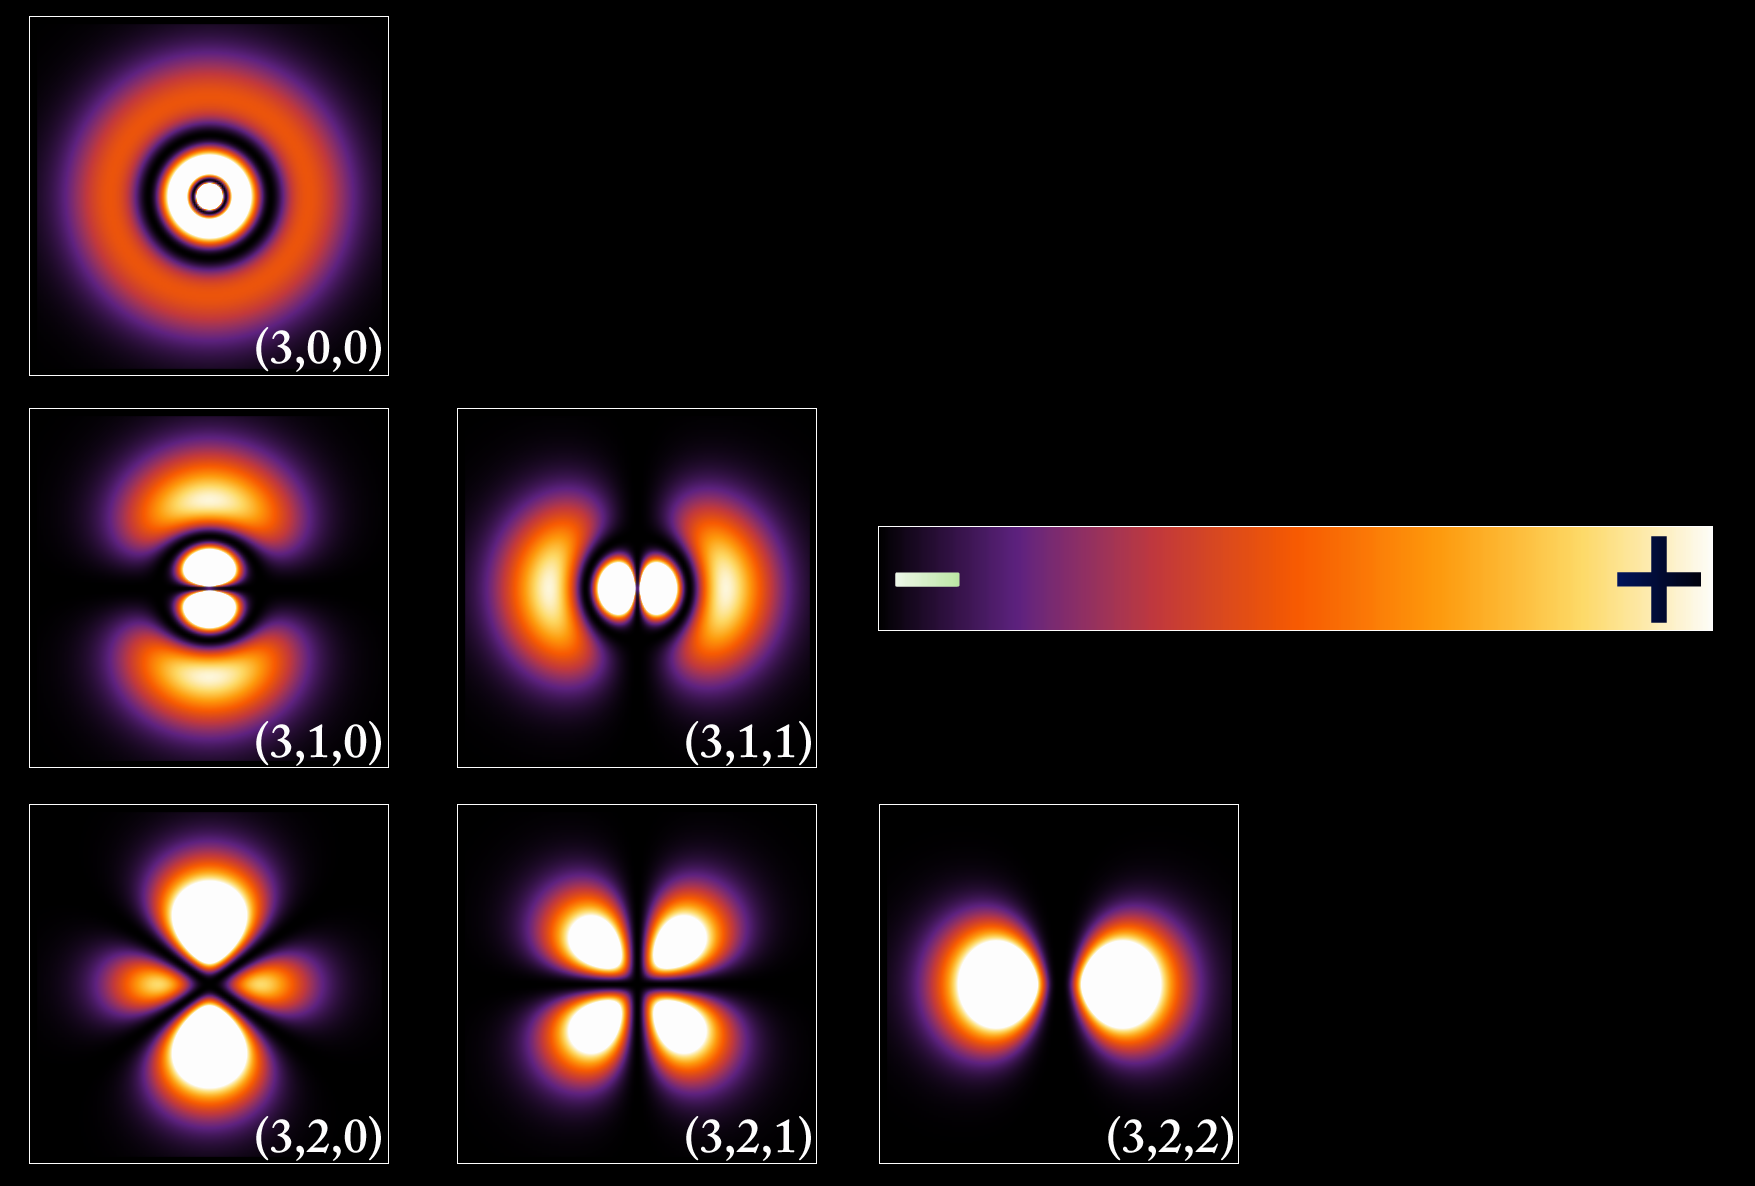
\includegraphics[width = 8.2cm]{Figures/3.HubbardModel/Hydrogen_Density_Plots.png}
\caption{Probability density plots for different hydrogen orbital wave functions corresponding to quantum numbers $(n, l, m)$ for $n = 3$. d-wave functions correspond to $l=2$. Note that the probability density is always higher in a region near the nucleus, and has a complicated shape, which will lead to a non-uniform distribution of electronic charge, as opposed to the case of the free electron gas.}
\end{figure}

Experimentally, $d-$electrons of transition metals show a hybrid behavior: sometimes they are accurately described by an ordinary band model, but there are occasions in which the atomic model is better. For example, we see spin wave phenomena in ferromagnetic transition metals, and the susceptibilities of some of these metals depend strongly on temperature. This is characteristic of an atomic (Heisenberg) model. On the other hand, the $d-$electrons contribute significantly to the low temperature specific heat and sometimes the magnetic moments per atom of some transition metal ferromagnets are not integer multiples of the Bohr magneton. This is characteristic of band theory\footnote{Think, for example, of a tight binding model. Electrons hop from atom to atom, and in general the spin of each atom depends on the particular electrons \say{belonging} to it at a given time. If we take an average of the total spin of each atom, we will in general not necessarily obtain an integer multiple of the Bohr magneton. If we simply had a collection of atoms, Hund's rule would apply, and each atom would have its spin aligned in a given direction. The average spin would then tend to be an integer multiple of the Bohr magneton.}. Our theory of correlations should describe this balance between band-like and atomic-like behavior.

The atomic picture of a solid consists of an electron gas where ions are immersed. The ions then interact in much the same way as they do in salts. This extreme scenario is surely not even close to the true state of affairs since the number of $d-$electrons per atom is in general not an integer. This motivates us to introduce a less restrictive model, which is not too far from the atomic model. We shall assume that while $d-$electrons still have some band motion, they are strongly correlated with each other so that the metal retains some atomic-like behavior. The correlations between electrons on different atoms are likely much weaker and we neglect them.

Let us now look at an example of the aforementioned circumstance. Take a partially filled $d-$band of non-interacting electrons. The spin of any given atom in the solid is just the total spin of all electrons on that atom. It fluctuates both in magnitude and in direction, with a characteristic time that depends on how frequently $d-$electrons hop (in the loose quantum mechanical sense). We can estimate the time interval between $d-$electron hopping events between atoms as a being of the order $\frac{\hbar}{\Delta}$, where $\Delta$ is the $d-$electron bandwidth. The spin can thus be thought of as being associated to each individual moving $d-$electron.

How do the electron interactions affect this picture? We start by recalling Hund's rule: the nature of the  interactions between atoms leads to an alignment of the spins on each atom. Since the atomic picture seems to prevail in our metal, we have reason to expect a similar effect to occur. An atom with a total spin in some direction at a given time will tend to attract electrons with the spin on that direction and repel those with opposite spin. This mechanism makes it unlikely for the spin of an atom to change much over time.

If the interactions between atoms are strong enough, the correlations become considerable, and to state it more precisely, the total spin of an atom will persist for a time that is long compared with the $d-$electron hopping time. Note that it is not the localization of the electrons that causes the spin state of the atom to persist. The specific electrons belonging to a given atom change all the time as long as their spin is consistent with the total spin requirement imposed by Hund's rule. For strong enough correlations, we may think of the spin as being associated to each atom, which opens up the possibility to describe the system using an atomic Heisenberg model.

A theory of electron correlations in a narrow energy band should reduce to an atomic model in the appropriate limit, for example atoms that are so far apart on a lattice that they interact only very weakly. Although we always keep in mind that we are focusing on $d-$electrons, we shall consider $s-$electrons in what follows for the sake of simplicity. The important conclusions will not differ significantly. We will use the atomicity of the electronic distribution to introduce an approximate representation of the electron interaction. It turns out that this representation is mathematically much simpler to handle than the Coulomb interaction itself.

In short, our picture is the following: electrons hop rapidly from atom to atom in a band-like fashion, but their motion is correlated in such a way that atomic characteristics emerge. The extent of atomic behavior depends, of course, on the strength of the interaction.

\subsection{Hubbard Hamiltonian}\label{hubbardHamiltonian}

Imagine a hypothetical partially filled narrow $s-$band with $n$ electrons per atom. Suppose you have obtained Bloch wave functions $\psi_{\bm k}$ corresponding to energies $\varepsilon_{\bm k}$ by solving the Schr\"odinger equation for some spin-independent mean field Hartree-Fock potential that accounts for the average interaction of the $s-$band electrons with electrons on other bands, and the interaction with the other $s-$electrons. The electrons on the band evolve according to the Hamiltonian (in a suitable unit system):

\begin{equation}\label{eq:startingHamiltonian}
\begin{split}
&\mathcal{H} = \sum_{\bm k \sigma} \varepsilon_{\bm k} c_{\bm k \sigma}^\dagger c_{\bm k \sigma} + \\
&\frac{1}{2} \sum_{ \substack{\bm k_1 \bm k_2 \\ \bm k_1' \bm k_2' \\ \sigma_1 \sigma_2 } } \left\langle \bm k_1 \bm k_2 \bigg| \frac{e^2}{r} \bigg| \bm k_1' \bm k_2' \right\rangle 
 c_{\bm k_1 \sigma_1}^\dagger c_{\bm k_2 \sigma_2}^\dagger c_{\bm k_2' \sigma_2} c_{\bm k_1' \sigma_1} \\
 &- \sum_{ \substack{\bm k \bm k' \\ \sigma} } \bigg[ 2 \left\langle \bm k \bm k' \bigg| \frac{e^2}{r} \bigg| \bm k \bm k' \right\rangle - \left\langle \bm k \bm k' \bigg| \frac{e^2}{r} \bigg| \bm k' \bm k \right\rangle \bigg] \nu_{\bm k'} c_{\bm k \sigma}^\dagger c_{\bm k \sigma} ,
\end{split}
\end{equation}
where the $\bm k-$sums run over the first Brillouin zone. The integrals are defined by

\begin{equation}\label{eq:integrals}
\begin{split}
&\left\langle \bm k_1 \bm k_2 \bigg| \frac{e^2}{r} \bigg| \bm k_1' \bm k_2' \right\rangle \equiv V^{\bm k_1 \bm k_2}_{\bm k_1' \bm k_2'}  =  \\
&e^2 \int \frac{\psi_{\bm k_1}^\star (\bm x) \psi_{\bm k_1'} (\bm x) \psi_{\bm k_2}^\star (\bm x') \psi_{\bm k_2'}(\bm x') }{| \bm x - \bm x' |} d\bm x d\bm x'
\end{split}
\end{equation}

The first term represents the band energies of the electrons and the second term represents the interactions among them. The last term subtracts the potential energy of the electrons in the part of the Hartree-Fock field due to the electrons of the $s-$band itself. This term ensures that we do not count the interactions of the electrons of the band twice: the Hartree-Fock field that specifies $\varepsilon_{\bm k}$ is computed taking into account these interactions, so if we didn't subtract the last term, we would count the energy of these interactions twice since they reappear in the second term. Furthermore, we assume that up and down spins are occupied equally, and $\nu_{\bm k}$ are the occupation numbers of the states of the band in the Hartree-Fock calculation. 

The term that we subtract in equation ($\ref{eq:startingHamiltonian}$) corresponds to the part of the interaction term which is already accounted for by the first diagonal mean field term. Thus, it corresponds to the mean field expansion of the interaction term (i.e. the second term), which is generically written

\begin{equation}
V_{\text{int}} = \frac{1}{2} V^{\nu\mu}_{\nu'\mu'} c_\nu^\dagger c_\mu^\dagger c^{\mu'} c^{\nu'} ,
\end{equation}
where the summation over repeated indices is implied.

We start by noting that in mean field, this quartic term becomes a sum of all possible 2-body terms (note that terms of the type $\left\langle cc \right\rangle$ and $\left\langle c^\dagger c^\dagger \right\rangle$ must vanish.

\begin{equation}\label{eq:c_mft}
\begin{split}
&c_\nu^\dagger c_\mu^\dagger c_{\mu'} c_{\nu'} \approx - \left\langle c_\nu^\dagger c_{\mu'} \right\rangle  c_{\mu}^\dagger c_{\nu'} - \left\langle c_{\mu}^\dagger c_{\nu'} \right\rangle c_{\nu}^\dagger c_{\mu'} + \\
&+ \left\langle c_{\nu}^\dagger c_{\nu'} \right\rangle  c_{\mu}^\dagger c_{\mu'} + \left\langle c_{\mu}^\dagger c_{\mu'} \right\rangle  c_{\nu}^\dagger c_{\nu'} ,
\end{split}
\end{equation}
where we ignored the constant terms which are unimportant in the Hamiltonian, in what concerns the dynamics. This Hartree-Fock mean field approximation is slightly tricky to show. It requires one to be precise about what the meaning of the mean field approximation is in terms of creation and annihilation operators. In mean field theory, we assume that the operator

\begin{equation}
\rho_{\mu\mu'} = c_{\mu}^\dagger c_{\mu'}
\end{equation}
is close to its average, so that we neglect second order terms in the fluctuations $\delta \rho_{\mu\mu'}$, i.e. $\rho_{\mu\mu'}$ is \say{large} only when its average is nonzero, otherwise it is negligibly small. Thus, for most combinations of indices, this operator will vanish. We follow the usual mean field procedure of writing the original operator as a deviation plus an average

\begin{equation}\label{eq:hartree}
c_{\nu}^\dagger \bigg( c_\mu^\dagger c_{\mu'} - \left\langle c_\mu^\dagger c_{\mu'} \right\rangle \bigg) c_{\nu'} + c_{\nu}^\dagger c_{\nu'} \left\langle c_\nu^\dagger c_{\nu'} \right\rangle
\end{equation}

Then we note that if $\nu' \neq \mu$, we can commute $c_{\nu'}$ with the parenthesis. But this is true except in a set of measure zero. In the thermodynamic limit $N \rightarrow \infty$, the number of allowed $\bm k$-states is very large, and if we take a continuum limit in which the set of possible $\bm k$-states becomes dense, then the commutation becomes exact. Repeating the procedure of writing (\ref{eq:hartree}) replacing $c_\nu^\dagger c_{\nu'} \mapsto c_\nu^\dagger c_{\nu'} - \left\langle c_\nu^\dagger c_{\nu'} \right\rangle + \left\langle c_\nu^\dagger c_{\nu'} \right\rangle $, we obtain

\begin{equation}
\begin{split}
&\underbrace{\big( c_\nu^\dagger c_{\nu'} - \left\langle c_\nu^\dagger c_{\nu'} \right\rangle \big) \big( c_\mu^\dagger c_{\mu'} - \left\langle c_\mu^\dagger c_{\mu'} \right\rangle \big)}_{\propto \, \delta \rho_{\mu\mu'} \, \delta \rho_{\nu\nu'} \rightarrow 0} + c_\nu^\dagger c_{\nu'} \left\langle c_\mu^\dagger c_{\mu'} \right\rangle \\
&+ c_\mu^\dagger c_{\mu'} \left\langle c_\nu^\dagger c_{\nu'} \right\rangle - \left\langle c_\mu^\dagger c_{\mu'} \right\rangle \left\langle c_\nu^\dagger c_{\nu'} \right\rangle
\end{split}
\end{equation}

But this result is not complete. This is only the so called Hartree or direct term. Due to identical nature of the interacting electrons, we must consider an analogous contribution for $\left\langle c_\nu^\dagger c_{\mu'} \right\rangle$ finite. We start by exchanging the first two operators: 

\begin{equation}
c_\nu^\dagger c_\mu^\dagger c_{\mu'} c_{\nu'} = - c_\mu^\dagger c_\nu^\dagger c_{\mu'} c_{\nu'}
\end{equation}
Then we proceed in exactly the same manner as before. The result is analogous, but a minus sign appears and we must switch $\mu \leftrightarrow \nu$:

\begin{equation}
- c_\mu^\dagger c_{\nu'} \left\langle c_\nu^\dagger c_{\mu'} \right\rangle \\
- c_\nu^\dagger c_{\mu'} \left\langle c_\mu^\dagger c_{\nu'} \right\rangle + \left\langle c_\nu^\dagger c_{\mu'} \right\rangle \left\langle c_\mu^\dagger c_{\nu'} \right\rangle
\end{equation}

Ignoring the constant terms of the type $\left\langle c^\dagger c \right\rangle \left\langle c^\dagger c \right\rangle$, we recover equation (\ref{eq:c_mft}).

Now we can simply substitute the mean field expansion of equation (\ref{eq:c_mft}) in the second term to  obtain the last term that is subtracted in equation (\ref{eq:startingHamiltonian}) (we omit the boldface on the $\bm k$'s solely in the following equation, but keep in mind that they are vectors):

\begin{equation}\label{eq:mean_field}
\begin{split}
&\frac{1}{2} \sum_{\substack{ k_1 k_2 k_1' k_2' \\ \sigma_1 \sigma_2} } V^{k_1 k_2}_{k_1' k_2'} \bigg( - \underbrace{\left\langle c_{k_1 \sigma_1}^\dagger c_{k_2' \sigma_2} \right\rangle}_{\delta_{k_1 k_2'} \delta_{\sigma_1 \sigma_2} \nu_{k_1} } c_{k_2 \sigma_2}^\dagger c_{k_1' \sigma_1} \\
& - \underbrace{\left\langle c_{k_2 \sigma_2}^\dagger c_{k_1' \sigma_1}  \right\rangle}_{\delta_{k_2 k_1'} \delta_{\sigma_1 \sigma_2} \nu_{k_2} } c_{k_1 \sigma_1}^\dagger c_{k_2' \sigma_2} + \underbrace{\left\langle c_{k_1 \sigma_1}^\dagger c_{k_1' \sigma_1} \right\rangle}_{\delta_{k_1 k_1'} \nu_{k_1} } c_{k_2 \sigma_2}^\dagger c_{k_2' \sigma_2}  \\
& + \underbrace{\left\langle c_{k_2 \sigma_2}^\dagger c_{k_2' \sigma_2} \right\rangle}_{\delta_{k_2 k_2'} \nu_{k_2} } c_{k_1 \sigma_1}^\dagger c_{k_1' \sigma_1} \bigg)\\
\end{split}
\end{equation}

In the language of Hartree Fock theory, the first two terms give the exchange term, and the last two terms the direct term. Apart from the $\frac{1}{2}$ factor, the term in (\ref{eq:mean_field}) becomes

\begin{equation}
\begin{split}
&- \sum_{\substack{k_1 k_2 \\ k_1' \sigma_1}} V_{k_1' k_1}^{k_1 k_2} \nu_{k_1} c_{k_2 \sigma_1}^\dagger c_{k_1' \sigma_1}  - \sum_{\substack{k_1 k_2 \\ k_2' \sigma_1}} V_{k_2 k_2'}^{k_1 k_2} \nu_{k_2} c_{k_1 \sigma_1}^\dagger c_{k_2' \sigma_1} \\
&+ \sum_{\substack{k_1 k_2 k_2' \\ \sigma_1 \sigma_2}} V_{k_1 k_2'}^{k_1 k_2} \nu_{k_1} c_{k_2 \sigma_2}^\dagger c_{k_2' \sigma_2}  + \sum_{\substack{k_1 k_2 k_1' \\  \sigma_1 \sigma_2}} V_{k_1' k_2'}^{k_1 k_2} \nu_{k_2} c_{k_1 \sigma_1}^\dagger c_{k_1' \sigma_1} \\
&= \sum_{k_1 k_2 \sigma_1} \bigg( 4 V_{k_1 k_2}^{k_1 k_2} - 2  V_{k_2 k_1}^{k_1 k_2}  \bigg) \nu_{k_2} c_{k_1 \sigma_1}^\dagger c_{k_1 \sigma_1}
,
\end{split}
\end{equation}
where we used momentum conservation to eliminate a $k'$-sum. Moreover, we used that the sum on spin ($\pm 1/2$) on the last two terms gives factors of 2 , since the interaction is spin independent and thus no spin-dependent term remains after we use momentum conservation. Making $k_1 \rightarrow k , \, k_2 \rightarrow k', \, \sigma_1 \rightarrow \sigma$, and recalling the definition in equation (\ref{eq:integrals}), we obtain the result we sought.

Now consider the Wannier functions

\begin{equation}
\phi(\bm x) = N^{-1/2} \sum_{\bm k} \psi_{\bm k} (\bm x) , 
\end{equation}
where $N$ is the number of atoms. We may write $\psi_{\bm k}$ as a  combination of these Wannier functions localized at each atom.

\begin{equation}
\psi_{\bm k} (\bm x) = N^{-1/2} \sum_i e^{i \bm k \cdot \bm R_i} \phi (\bm x - \bm R_i) ,
\end{equation}
where the sum runs over all atomic positions $\bm R_i$. Introducting the annihilation (creation) operators of an electron of spin $\sigma$ in the orbital state $\phi (\bm x - \bm R_i)$ (at site $i$), $c_{i\sigma}^{(\dagger)}$, we may write

\begin{equation}
c_{\bm k \sigma}^{(\dagger)} = N^{-1/2} \sum_i e^{i \bm k \cdot \bm R_i} c_{i\sigma}^{(\dagger)}
\end{equation}

Thus, the Hamiltonian becomes 

\begin{equation}
\begin{split}
&\mathcal{H} = \sum_{\substack{ i j \\ \sigma} } K_{ij} c_{i \sigma}^\dagger c_{j \sigma} + \\
&\frac{1}{2} \sum_{\substack{i j k l \\ \sigma \sigma'} }\left\langle i j \bigg| \frac{e^2}{r} \bigg| k l \right\rangle 
 c_{i \sigma}^\dagger c_{j \sigma'}^\dagger c_{l \sigma'} c_{ k \sigma} \\
 &- \sum_{\substack{ijkl \\ \sigma }} \bigg[ 2 \left\langle i j \bigg| \frac{e^2}{r} \bigg| k l \right\rangle - \left\langle i j \bigg| \frac{e^2}{r} \bigg| l k \right\rangle \bigg] \nu_{j l} c_{i \sigma}^\dagger c_{ k \sigma} ,
\end{split}
\end{equation}
where

\begin{equation}\label{eq:hopping_matrix}
K_{ij} = N^{-1} \sum_{\bm k} \varepsilon_{\bm k} e^{i \bm k \cdot ( \bm R_i - \bm R_j )},
\end{equation}
and

\begin{equation}
\nu_{j l} = N^{-1} \sum_{\bm k} e^{i \bm k \cdot ( \bm R_j - \bm R_l) }
\end{equation}

Now comes the crucial approximation. For a narrow energy band, the Wannier functions $\phi$ nearly coincide with atomic $s-$functions. For small bandwidth these $s-$functions form an atomic shell whose radius is small compared with the spacing between atoms (or lattice constant). Thus, the integral $U = \left\langle i i \big| e^2 / r \big| i i \right\rangle$ should be much larger than all other integrals. This suggests the seemingly crude approximation of neglecting all other integrals. It turns out that this approximation is not so radical as it could seem at first sight since the other integrals are indeed much smaller than $U$. In fact, they are smaller by about two orders of magnitude for $3d$ electrons of transition metals \cite{Hubbard1963}. We end up with

\begin{equation}
\mathcal{H} = \sum_{i, j, \sigma} K_{ij} c_{i\sigma}^\dagger c_{j\sigma} + \frac{U}{2} \sum_{i\sigma} n_{i\sigma} n_{i, -\sigma} - U \sum_{i, \sigma} \nu_{i, i} n_{i, \sigma}
\end{equation}
where $n_{i\sigma} = c_{i\sigma}^\dagger c_{i\sigma}$. Note that $\nu_{i, i} = N^{-1} \sum_{\bm k} \nu_{\bm k} = n/2$, which means that the last term is constant and may be dropped. Now, the hopping matrix $\bm K$ should be found by inverse Fourier transforming the dispersion relation $\varepsilon_{\bm k}$.

In general, we have a well defined crystal wavevector that depends on the symmetry of the lattice, which may be written as the Fourier transform

\begin{equation}
\left| \bm k \right\rangle \equiv \frac{1}{N} \sum_{\bm r} e^{i\bm k \cdot \bm r} \left| \bm r \right\rangle
\end{equation}

Recalling the form of the hopping Hamiltonian

\begin{equation}
\mathcal{H}_{\text{hop}} = - \sum_{\bm r \bm r'} K (\bm r - \bm r') \left| \bm r' \right\rangle \left\langle \bm r \right|
\end{equation}
we can obtain the dispersion relation.

\begin{equation}
\begin{split}
- \mathcal{H}_{\text{hop}} \left| \bm k \right\rangle &= \frac{1}{\sqrt{N}} \sum_{\bm r \bm r'} K ( \bm r - \bm r' ) e^{i \bm k \cdot \bm r} \left| \bm r' \right \rangle \\
&= \frac{1}{\sqrt{N}} \bigg( \sum_{\bm R} K(\bm R) e^{i\bm k \cdot \bm R} \bigg) \bigg( \sum_{\bm r'} e^{i\bm k \cdot \bm r'} \left| \bm r' \right\rangle \bigg) \\
& = \varepsilon_{\bm k} \left| \bm k \right\rangle
\end{split}
\end{equation}
and here we recognize the dispersion relation as the (negative) Fourier transform of the hopping

\begin{equation}
\varepsilon_{\bm k} = - \sum_{\bm R} K(\bm R) e^{i\bm k \cdot \bm R} 
\end{equation}

This gives us an interpretation of the $\bm K$ matrix: given the dispersion relation for a tight binding model, if we take the inverse Fourier transform we obtain the matrix elements $K_{i j}$.

Let's suppose we have the simplest uniform nearest neighbor hopping model. Going back to equation (\ref{eq:hopping_matrix}), and recalling that the sum on $\bm k$ is restricted to the first Brillouin zone, we obtain the usual tight binding result: $K_{\left\langle i j \right\rangle} = - t$ and $0$ otherwise (i.e. $\bm K$ is a very sparse matrix that is only non-zero for $i, j$ nearest neighbors). The Hubbard Hamiltonian is then

\begin{equation}\label{eq:hubbard_hamiltonian}
\mathcal{H} = - t \sum_{\left\langle i, j \right\rangle, \sigma} \bigg(c_{i,\sigma} c_{j,\sigma}^\dagger + c_{j,\sigma} c_{i,\sigma}^\dagger \bigg) + U \sum_{i} n_{i,\uparrow} n_{i\downarrow}
\end{equation}